% !TEX encoding = UTF-8 Unicode 
% !TEX root = praca.tex

\chapter{Opis systemu}

Rozdział ten poglądowo opisuje system będący przedmiotem pracy, z naciskiem na 
architekturę oprogramowania i projektowanie systemów. 
Poszczególne elementy systemu zostały przedstawione na schemacie poglądowym na rys. \ref{fig:hl_sys}.

\begin{figure}[h!]
    \centering 
    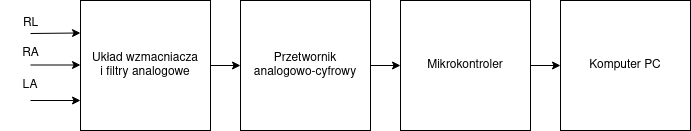
\includegraphics[scale=0.6]{pl/media/hl_system.png}
    \caption{Schemat poglądowy systemu}
    \label{fig:hl_sys}
\end{figure}

Do pomiaru aktywności elektrycznej serca zastosowano klasyczny układ 3 elektrod pomiarowych używany często
w diagnostyce arytmii \cite{FRANCIS201692}, z oznaczeniami \textit{RL} (\textit{right leg}, prawa noga), 
\textit{RA} (\textit{right arm}, prawa ręka) oraz \textit{LA} (\textit{left arm}, lewa ręka). W tej 
konfiguracji elektrody można umieścić w sposób jaki sugerują oznaczenia tzn. na kończynach lub alternatywnie 
na klatce piersiowej (\textit{RA} i \textit{LA}) oraz poniżej żeber (\textit{RL}). 
Kolejność elektrod można zamieniać aby uzyskać inne konfiguracje również umożliwiające akwizycję sygnału
mającego wartość w diagnostyce.

\begin{figure}[h!]
    \centering 
    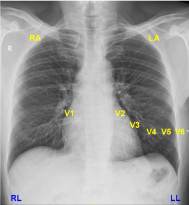
\includegraphics[scale=1]{pl/media/electrodes.png}
    \caption{Zdjęcie rentgenowskie klatki piersiowej wraz z oznaczeniami\\ dla 3-elektrodowej konfiguracji oraz oznaczeniami dodatkowymi
    \cite{FRANCIS201692}(\textit{Fig. 1.})}
    \label{fig:ele}
\end{figure}

\newpage

\section{Wzmocnienie sygnału i filtracja analogowa}

Sygnał \textit{EKG} charakteryzuje się małymi amplitudami, w zakresie od dziesiątek do setek $\mu V$ \cite{Zywietz1990}.
Ta cecha badanego sygnału uniemożliwia dokonywanie pomiaru w sposób dokładny przez klasyczne przetworniki analogowo/cyfrowe (\textit{ADC}, ang. \textit{Analog to Digital Converter})
ze względu na ich niską rozdzielczość. Jako rozwiązanie w pracy zastosowano zestaw wzmacniaczy w układzie scalonym firmy \textit{Analog Devices}, \textit{AD8232} \cite{AD8232ds}. 
Ze względu na to że mierzone impulsy mogą mieć wartości ujemne, \textit{AD8232} przesuwa wzmacnia i normalizuje amplitudę sygnału do przedziału $[0; 3,3V]$ co umożliwia 
próbkowanie i jego kwantyzację za pomocą klasycznych przetworników \textit{ADC}. 
\textit{AD8232} zapewnia również mechanizm wykrywania podłączonych elektrod (ang. \textit{leads off detection}).


W pracy użyto płytki drukowanej z układem \textit{AD8232} \cite{AD8232BS} w konfiguracji z dwoma pasywnymi filtrami analogowymi: 
górnoprzepustowym oraz dolnoprzepustowym, o wynikowym paśmie przepuszczania $[0,5 Hz; 40Hz]$ (rys. \ref{fig:afilt}) \cite{AD8232ds}.

\begin{figure}[h!]
    \centering 
    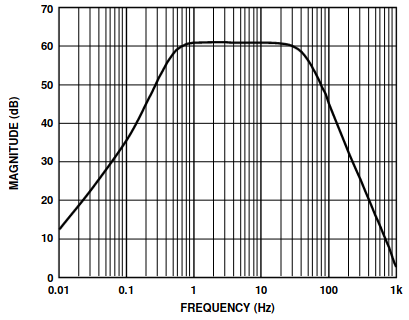
\includegraphics[scale=0.75]{pl/media/afilt.png}
    \caption{Wykres charakterystyki częstotliwościowej zastosowanego układu filtrów analogowych podany przez producenta \cite{AD8232ds}(\textit{Fig. 67.})}
    \label{fig:afilt}
\end{figure}

\newpage

\section{Próbkowanie i kwantyzacja}

